Benchmark tests are performed with the primary goal to measure the performance of the CPU for High Energy Physics applications. 
Alongside the legacy HEP-SPEC06 (HS06) benchmark \cite{Hepspec}, the performance of the compute resources is furthermore evaluated with the ATLAS Kit Validation
KV \cite{DeSalvo:2010zza}, a fast benchmark developed to provide real-time information of the WLCG performance and available in the CERN benchmark suite \cite{Alef:2017jyx}.
The primary target is to measure the performance of the CPU for High Energy Physics applications.
The KV benchmark is making use of the simulation toolkit GEANT4 \cite{Agostinelli:2002hh} to simulate the interactions of single muon events in the detector of the ATLAS experiment
and provides as ouput the number of events produced per second. It constitutes a realistic workload for High Energy Physics jobs. \\

To assess the impact of the virtualization, the performance of the identical hardware configuration (20 cores Intel Xeon E5-2630 CPUs) has been determined either deployed via
the standard bare metal operation on the \NEMO cluster (\NEMO bare metal) and on the ATLAS Tier-3 center in Freiburg (ATLAS Tier-3 bare metal), or as virtual machines on the
\NEMO cluster (\NEMO VM). On the ATLAS Tier-3 bare metal and on the virtual machines running on the \NEMO cluster, hyper-threading (HT) technology is activated. Both are using Scientific
Linux 6 \cite{SL6} as the operating system.
On the cluster \NEMO bare metal jobs are restricted to 20 cores by cgroups, since the application mix is broader than on HEP clusters. The operating system is CentOS7 \cite{CentOS7}.
The scores of the HEP-SPEC06 and KV benchmarks have been determined for these three configurations as a function of the number of cores actually used by the benchmarking processes.
This number ranges from 2 to 40 for the ATLAS Tier-3 bare metal and for the \NEMO VM, for which HT is enabled, and from 2 to 20 for the \NEMO bare metal, for which HT is not implemented.
The benchmarks have been run 20 times for each core multiplicity value, and the means and standard deviations of the corresponding distributions have been extracted. \\

\begin{figure}[htbp]
\centering
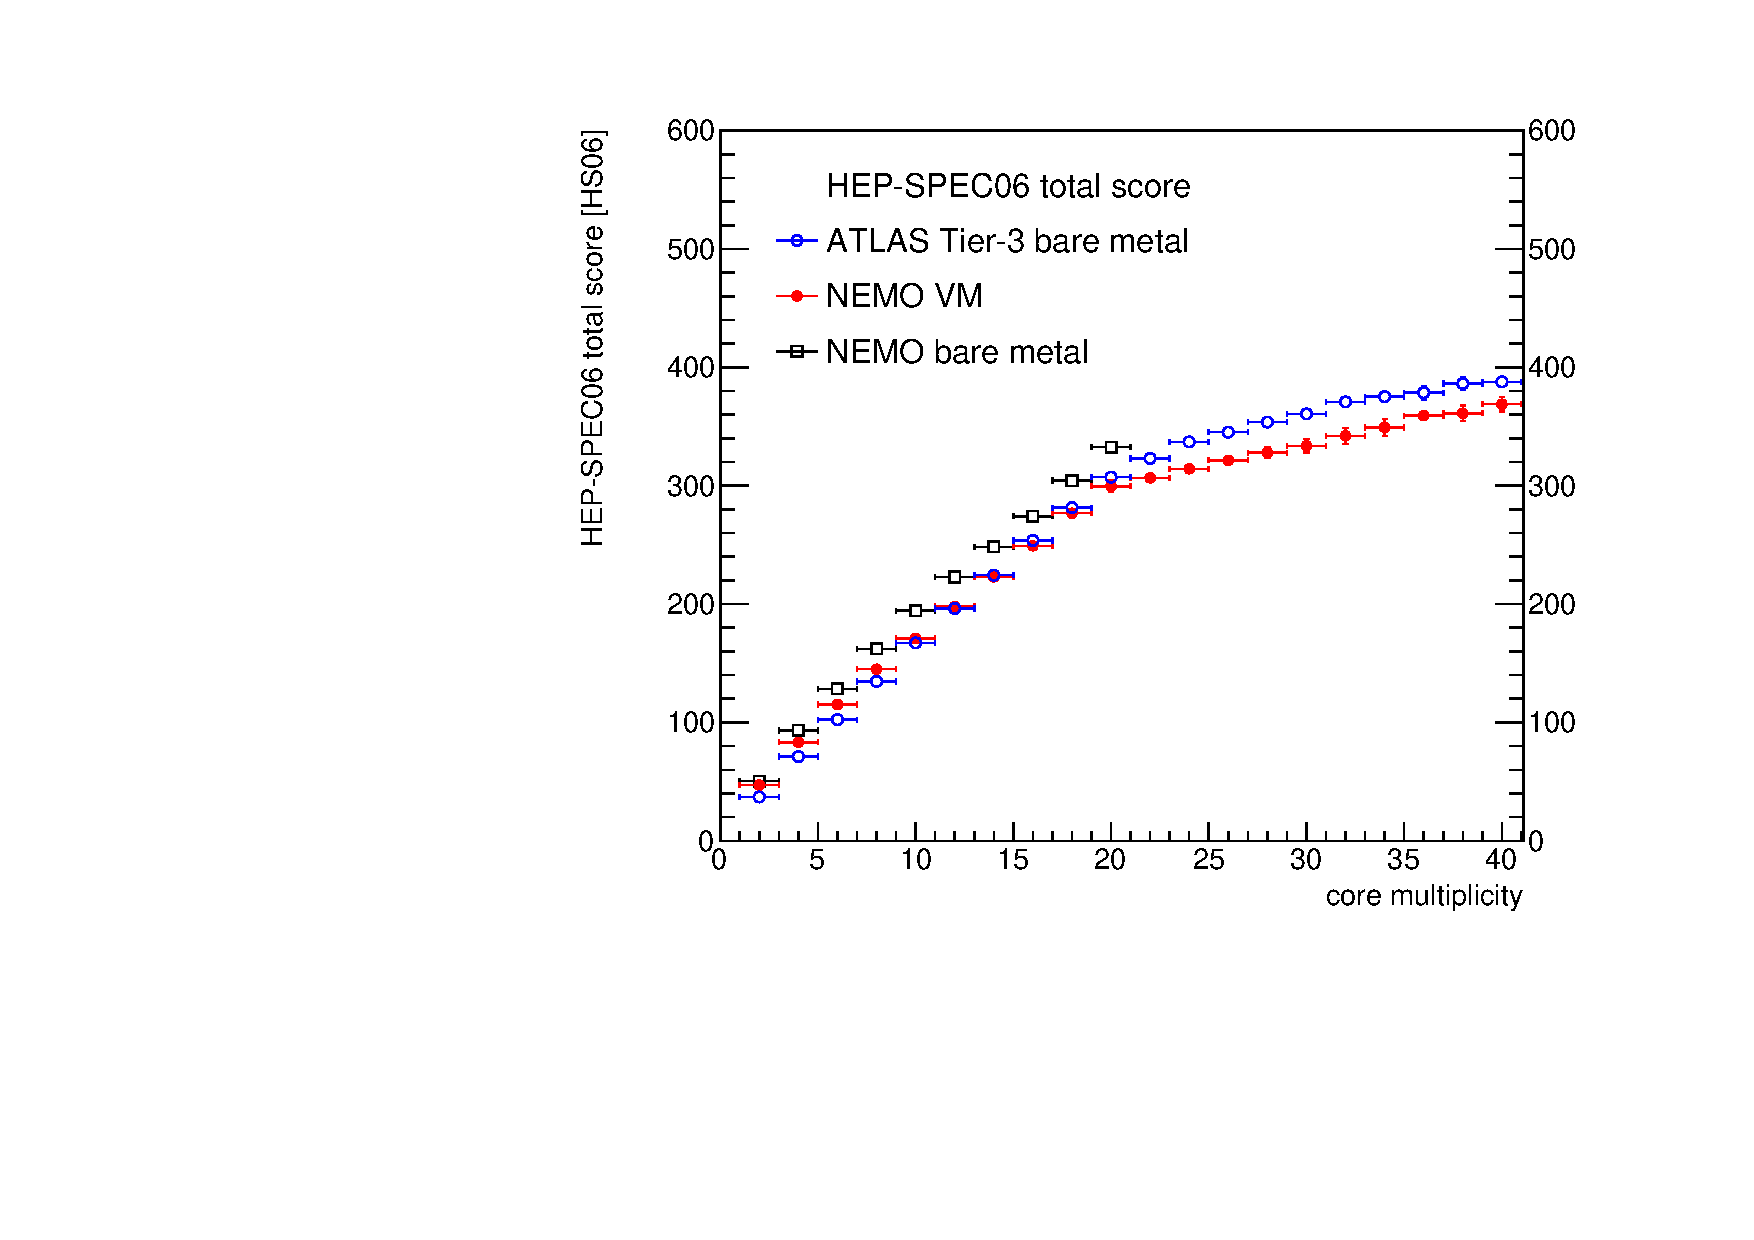
\includegraphics[width=0.44\textwidth]{figures/benchmark-hepspec06-total.pdf}
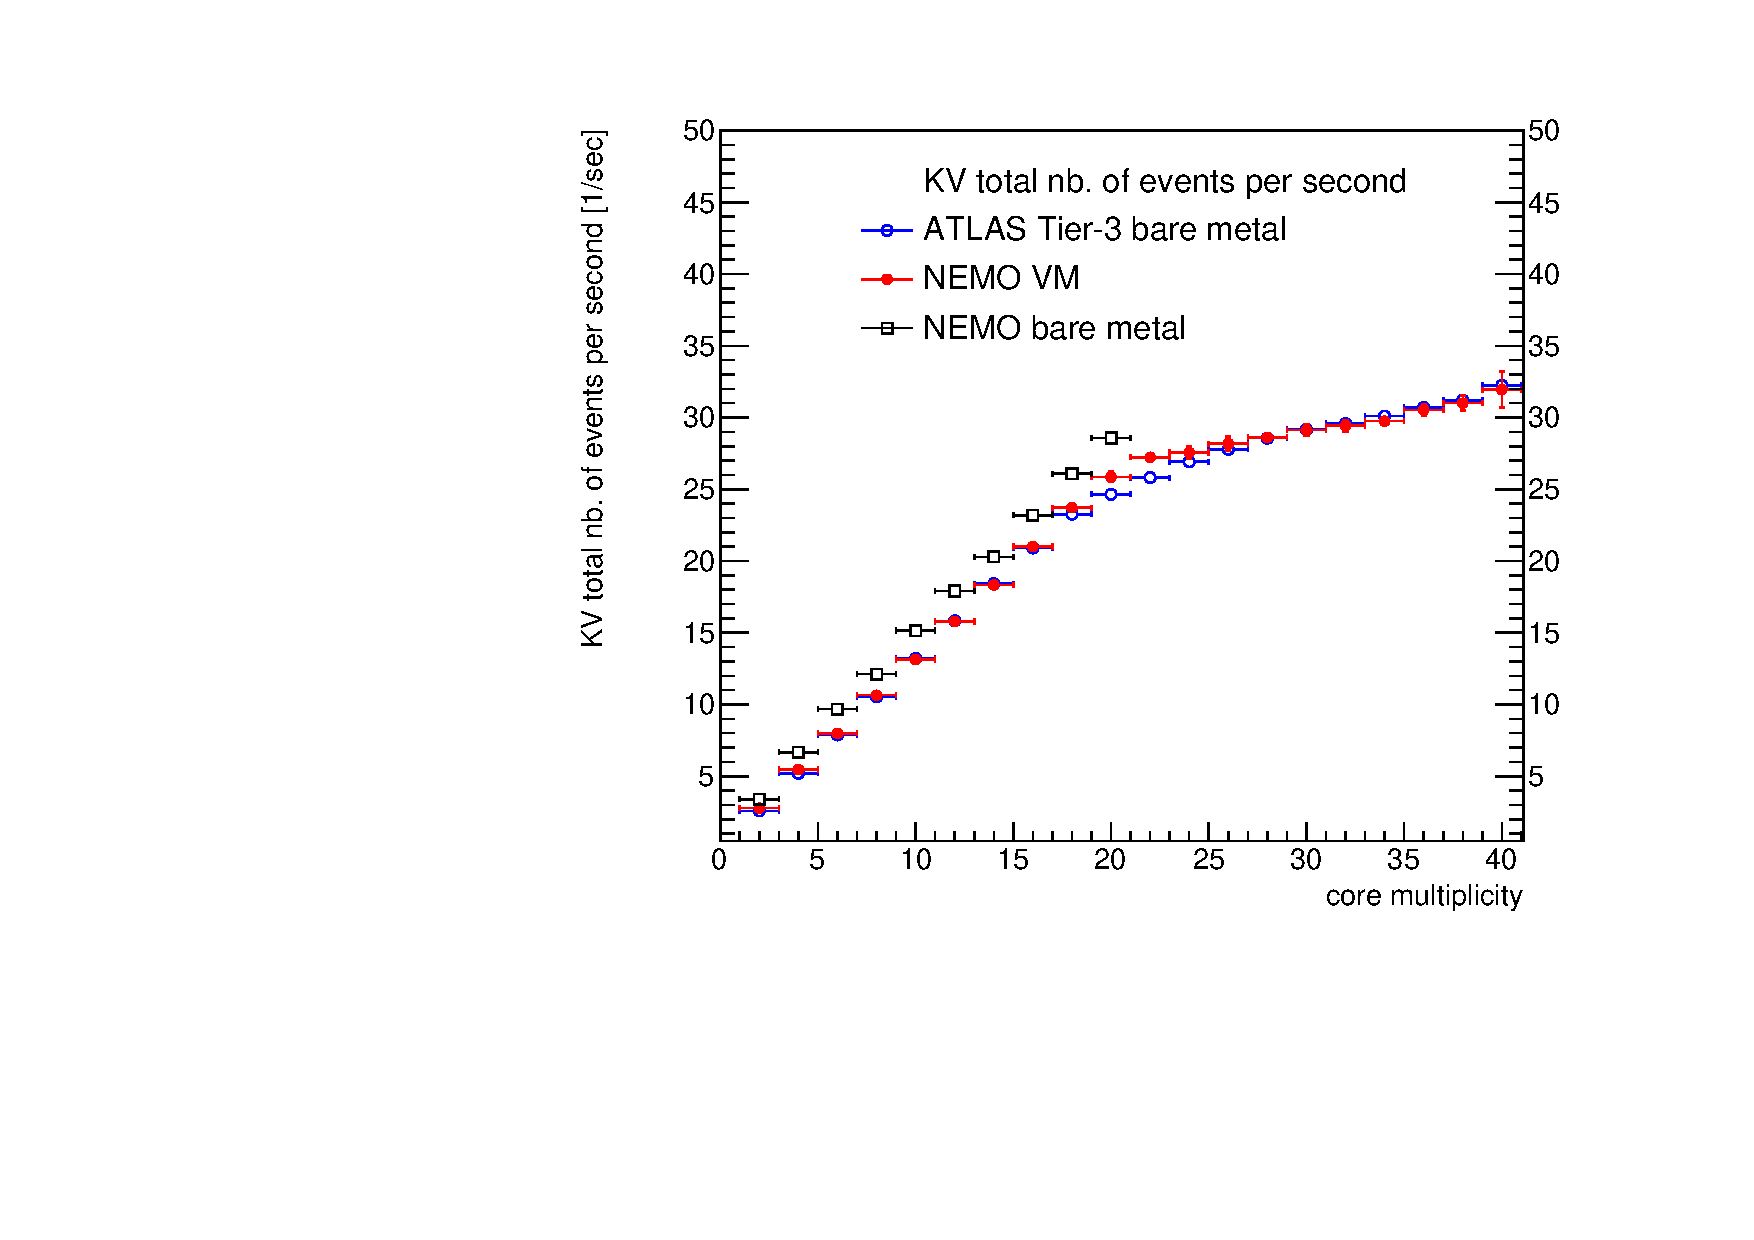
\includegraphics[width=0.44\textwidth]{figures/kv-BFG-BM-NEMO-VM-NEMO-BM-total.pdf} 
\caption{Total score as a function of the core multiplicity for the HEP-SPEC06 (top) and KV (bottom) benchmarks for the ATLAS Tier-3 bare metal (blue open circles),
the \NEMO VMs (red full circles) and the \NEMO bare metal (black open squares). The data points represent the average values of the benchmarks for each core multiplicity,
and the vertical bars show the associated standard deviations.}
\label{bmk-total}
\end{figure}

The HEP-SPEC06 and KV results are presented in Figure \ref{bmk-total} for the three configurations considered.
The total scores of the two benchmarks are increasing until the maximum number of physical cores has been reached, and are characterized by a flattening increase afterwards.
The scores of the virtual machines running on the \NEMO cluster are only slightly lower than those obtained for the \NEMO bare metal, and the loss of performance
due to the virtualization does not exceed 10$\%$.
For the VMs running on the \NEMO cluster and the ATLAS Tier-3 bare metal, the interplay between the virtualization and the different operating systems leads to very similar scores
for the two configurations, particularly for the KV benchmark, and the loss of performance is smaller than 10$\%$ as well.

% References for HEPSPEC
%%https://indico.cern.ch/event/49388/contributions/2014772/attachments/960838/1363966/20090127_NewCPUbenchmark_final.pdf
%%http://w3.hepix.org/benchmarking.html
%%https://spec.org/benchmarks.html
%%

%
%realistic load: as user
%machine reserved: root
%Hier sieht man, dass die Bare-Metal-User-Jobs wesentlich weniger performant sind, und die User-Jobs auf den VMs beinahe an die ROOT-Tests auf bare-metal herankommen. Interessant ist auch, dass bei den User-Jobs der Trend umgekehrt ist: Dort ist die HEPSPEC pro Core(!) etwas besser fuer 8 Cores. Es koennte aber auch sein, dass das bei den ROOT-Jobs auch so waere, dort haben wir die Zahlen in dem Bereich ja nicht.
%
